\begin{figure} [h]
\usetikzlibrary{shapes,arrows}

\tikzstyle{block} = [draw, rectangle, minimum height=3em, minimum width=6em]
\tikzstyle{input} = [coordinate]
\tikzstyle{output} = [coordinate]

\centering
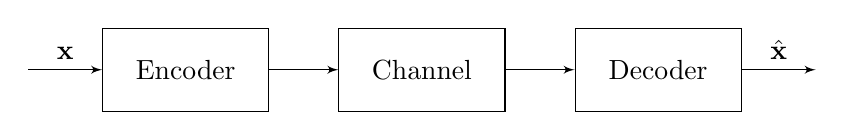
\begin{tikzpicture}[auto, node distance=2cm,>=latex']
\centering

    % We start by placing the blocks
    \node [input, name=input] {};    
    \node [block, right of=input] (encoder) {Encoder};
    \node [block, right of=encoder, node distance=3cm] (channel){Channel};
    \node [block, right of=channel, node distance=3cm] (decoder){Decoder};
    \node [output, right of=decoder] (output) {}; 
    
    
    \draw [->] (encoder) -- node[name=u] {} (channel);
    \draw [->] (channel) -- node[name=v] {} (decoder);
    \draw [draw,->] (input) -- node {$\textbf{x}$} (encoder);
    \draw [->] (decoder) -- node [name=y] {$\hat{\textbf{x}}$}(output);

\end{tikzpicture}
\caption{\textit{Simulation overview} \label{fig:simulationOverview}}
\end{figure}